%%%%%%%%%%%%%%%%%%%%%%%%%%%%%%%%%%%%%%%%%%%%%%%%%%%%%%%%%%%%%%%%%%%%%%%%%%%%%%%%
% exp-foraging.tex: Chapter with foraging experiment results for RQ1-RQ3.
%%%%%%%%%%%%%%%%%%%%%%%%%%%%%%%%%%%%%%%%%%%%%%%%%%%%%%%%%%%%%%%%%%%%%%%%%%%%%%%%
\chapter{Foraging Experiments}\label{chap:exp-foraging}
%%%%%%%%%%%%%%%%%%%%%%%%%%%%%%%%%%%%%%%%%%%%%%%%%%%%%%%%%%%%%%%%%%%%%%%%%%%%%%%%

\section{RQ1}\label{sec:exp-RQ1}

\section{RQ2}\label{sec:exp-RQ2}
For all experiments we average the results of 20 experimental runs of
$T = 10,000$ seconds. We define our cost measure $\CostFunc$ as the execution
time for a given task. We use a constant swarm density~\cite{Hamann2013} (ratio
of swarm size to arena area) of 10\%, which helps to minimize the effects of
increasing inter-robot interactions, allowing us to obtain more reliable
measures of our quantities of interest. That is, by using a constant swarm
density we maintain the same level of inter-robot interaction with increasing
swarm sizes, removing artifacts from increasing robot interaction levels from
the results, which would otherwise arise from variable density scenarios as
swarm size is increased.

We evaluate our derived methods against the following controllers from other
state-of-the-art literature~\cite{Harwell2018,Pini2011b,Pini2012}, summarized briefly
here:
%
\begin{itemize}
\item {\textit{Epsilon Greedy}, in which robots choose the task of least cost with
    probably $\epsilon$, and a random task otherwise; has a linear regret
    bound~\cite{Auer2002,Pini2013a,Pini2012}.}
\item {\textit{UCB1}, in which robots treat task allocation as a multi-armed bandit
    problem; has a logarithmic regret bound~\cite{Auer2002,Pini2013a,Pini2012}. }
\end{itemize}
%
\subsection{Effect on Performance of Task Decomposition Graph Richness }\label{sec:exp-tdgraph-richness}
%
To gain insight into the effect of task decomposition graph richness on
performance (and answer~\gls{RQ2.1}), we compare all methods on \emph{compound}
and \emph{complex} task decomposition graphs~\cite{Korsah2013}. We define a
\emph{swarm configuration} as an (X,Y) point corresponding to a specific
combination of swarm size and task allocation method. We compare and correlate
the levels of emergent intelligence and performance on both types of graphs
using the metric defined by~\cite{Harwell2019a}, which is a function of swarm
size and robot control algorithm. It computes the sub-linearity of increases in
inter-robot interference across either (1) linearly increasing swarm sizes, or
(2) task allocation methods. Linear or superlinear increases in interference
levels indicates more random and/or disorganized motion and therefore less
emergent intelligence.
%
\begin{figure}[!htbp]
 \centering
  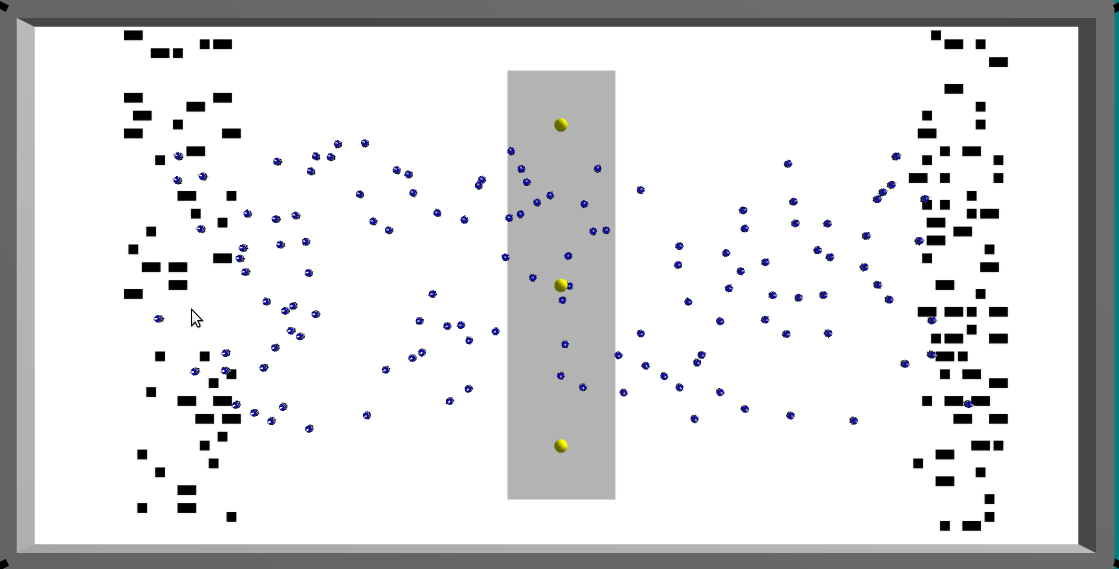
\includegraphics[width=.8\linewidth]{figures/chapter2/ds-foraging.png}
  \caption[Example dual source (DS) foraging scenario.]{\label{fig:ds-foraging}
    Multiple robots (blue blobs), objects to be collected (black squares), and
    the nest in the center (gray). }
\end{figure}
%
Previous work on task partitioning exclusively used single source foraging scenarios,
in which all objects are distributed in a single cluster within a rectangular
arena~\cite{Harwell2018,Harwell2019a,Ferrante2015,Pini2011b}. In this work we utilize
a \emph{dual source} foraging scenario, shown in Fig.~\ref{fig:ds-foraging}, in order
to provide swarms a richer environment to learn and exploit, as opposed to the
simpler single source environment.

\begin{figure}[!htbp]
  \centering
  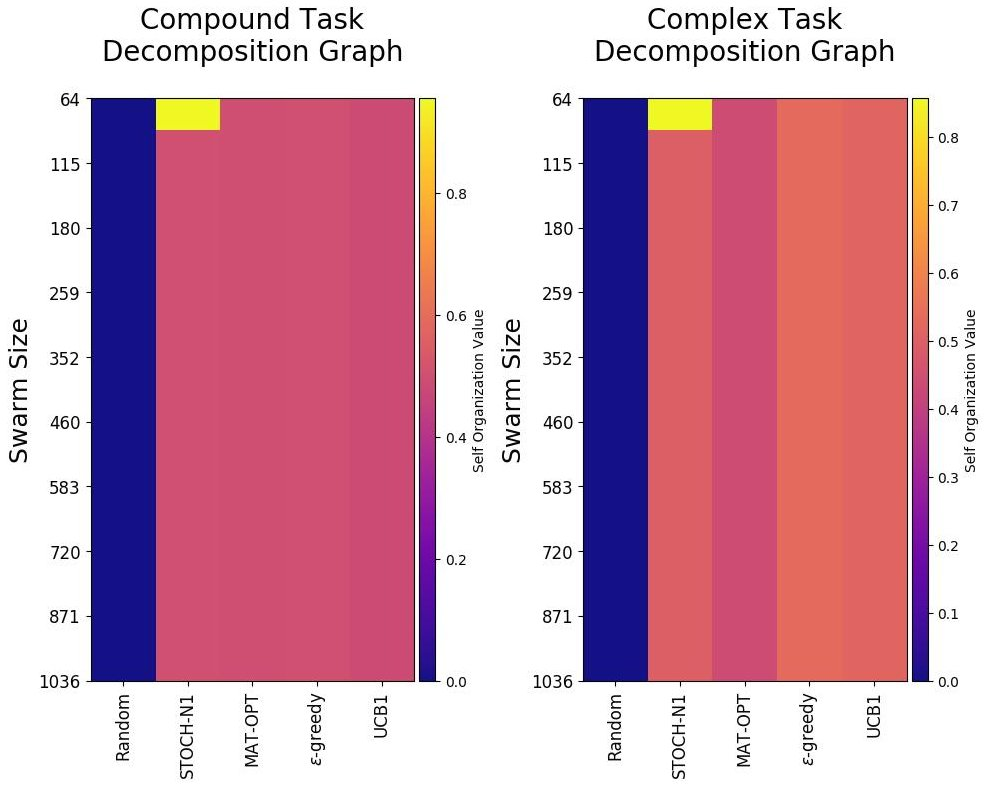
\includegraphics[width=8cm]{{figures/chapter2/cc-pm-self-org-fl-DS.36x18}.jpeg}
  \caption[Emergent intelligence via self-organization in DS scenario
  (\cref{fig:ds-foraging})]{\label{fig:DS-self-org} Using a 10\% swarm density
    under imperfect information. }
\end{figure}

\begin{figure}[!htbp]
  \centering
  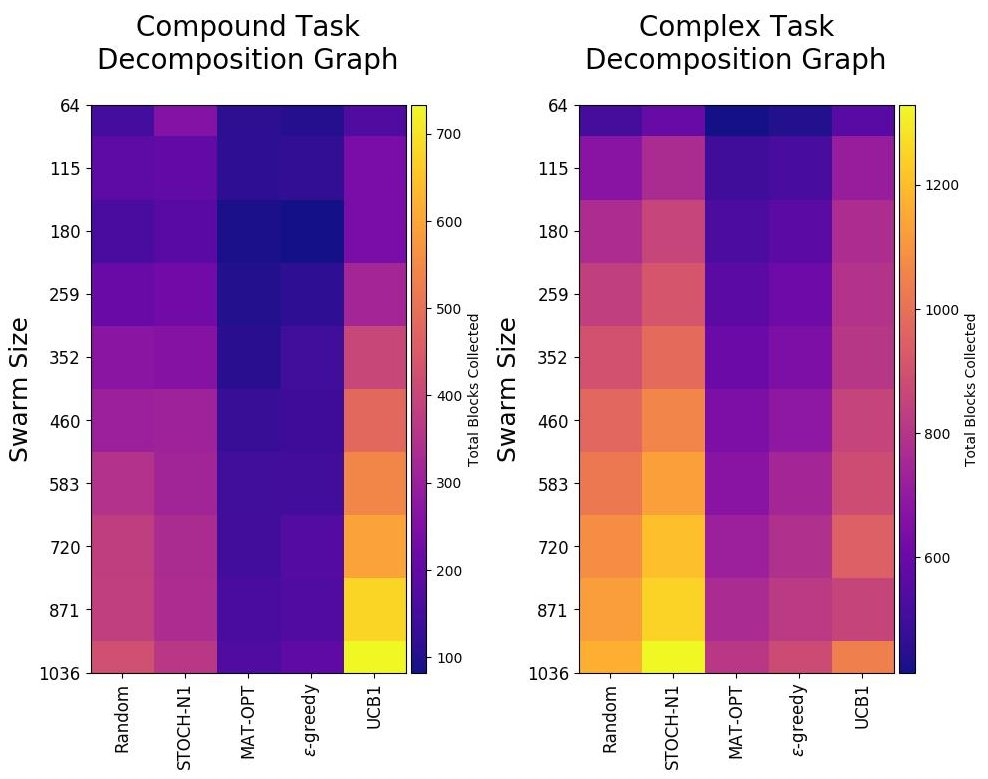
\includegraphics[width=8cm]{{figures/chapter2/cc-pm-blocks-transported-cum-DS.36x18}.jpeg}
  \caption[Performance in DS scenario
  (\cref{fig:ds-foraging})]{\label{fig:DS-perf} Using a 10\% swarm density under
    imperfect information.}
\end{figure}

From Fig.~\ref{fig:DS-self-org}, we see that the observed levels of self-organization
are uniformly higher for complex task decomposition graphs than for compound graphs
across all tested methods, even those not specifically designed to be sensitive to
task decomposition graph richness. The \gls{stoch-n1} method, which was specifically
designed to be sensitive to graph richness, has the highest emergent intelligence and
performance across all scales. Comparing Fig.~\ref{fig:DS-self-org} and
Fig.~\ref{fig:DS-perf} we observe that, generally speaking, higher levels of swarm
intelligence are positively correlated with higher performance.
%
\subsection{Emergence of Swarm Intelligence from Task Decomposition Graph Richness}
%
To investigate the origin of swarm emergent intelligence (\ref{research-Q2}), we ran
two additional sets of experiments. First, we enforce our matroid optimality
constraints by artificially injecting the swarm with perfect knowledge about evolving
task costs ($\CostFunc$) at every timestep. From our measurements (not shown), in
a~\textasciitilde{}1,000 robot swarm with a density of 10\%, no more than 3\% of
robots are engaged in collision avoidance at any given time, on average (for the
smaller swarms, it is much less), and $\CostFunc$ monotonicity is maintained. We
cannot guarantee multiple robots will not interact within a finite operating arena
(as strictly required to realize the \gls{mat-opt} task allocation space without task
dependencies), but our use of a low swarm density reduces the probability that
interactions will violate cost function monotonicity (e.g.,~obviating the occurrence
of excessive inter-robot interference at high densities).

\begin{figure}[!htbp]
  \centering
  \includegraphics[height=4cm]{figures/chapter2/{depth1-cc-pm-blocks-collected-cum-DS.36x18_01}.png}
  \caption[Performance difference comparison on a \emph{compound} task
  decomposition graph between swarms operating under matroid optimality
  constraints vs. relaxation.]{\label{fig:DS-relaxation-depth1} Negative values
    indicate that a performance drop was observed when constraints were relaxed,
    when compared with Fig.~\ref{fig:DS-perf}.\rule[-2ex]{0pt}{1ex}}
\end{figure}

We frame these results in terms of performance drops, comparing the drop in
performance when matroid optimality constraints are relaxed between two otherwise
identical swarms. In Fig.~\ref{fig:DS-relaxation-depth1}, \emph{negative} values
indicate a drop in performance, and \emph{positive} values indicate that swarms
operating under imperfect information performed better.  We see performance drops
consistently for both the \gls{mat-opt} and the $\epsilon$-greedy methods on the compound
task decomposition graph, in the neighborhood of \textasciitilde{}5\% as expected, as
they are the methods most sensitive task cost accuracy. The increased performance of
UCB1 under relaxation is somewhat anomalous, though we speculate that it could be due
to many robots allocating themselves the same sequence of tasks, which at larger
swarm sizes resulted in increased congestion at the shared caches. In
Fig.~\ref{fig:DS-relaxation-depth2}, we see much smaller scales of performance drops
in general, and more cases in which the swarm operating under perfect information
does \emph{better} than the one without it.

\begin{figure}[htb!]
  \centering
  \includegraphics[height=4cm]{figures/chapter2/{depth2-cc-pm-blocks-collected-cum-DS.36x18_01}.png}
  \caption[Performance difference comparison on a \emph{complex} task
  decomposition graph between swarms operating under matroid optimality
  constraints vs. relaxation.]{\label{fig:DS-relaxation-depth2} Negative values
    indicate that a performance drop was observed when constraints were relaxed,
    when compared with Fig.~\ref{fig:DS-perf}.}
\end{figure}

\section{RQ3}\label{sec:exp-RQ3}
